\documentclass[tikz,border=20pt]{standalone}
\usetikzlibrary{calc}

\begin{document}
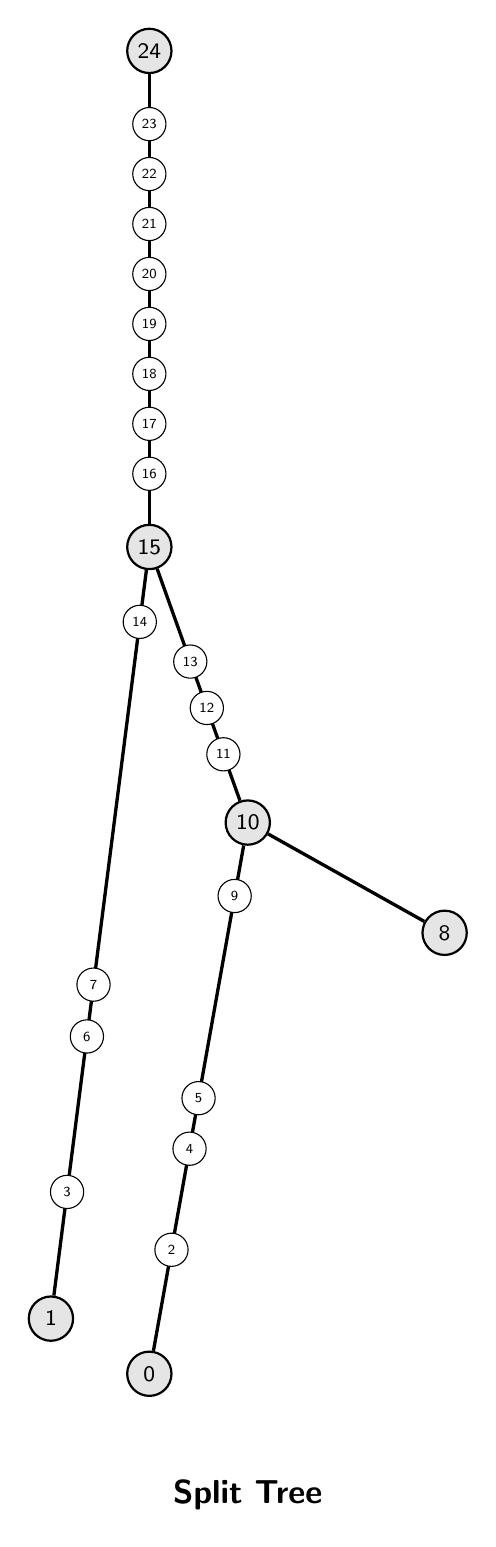
\begin{tikzpicture}[
    y=0.7cm, x=2.5cm,
    crit node/.style={circle, draw=black, fill=gray!20, thick, inner sep=1pt, minimum size=16pt, font=\sffamily\footnotesize},
    reg node/.style={circle, draw=black, fill=white, inner sep=0.5pt, minimum size=12pt, font=\sffamily\tiny},
    main edge/.style={very thick, draw=black}
]

% 关键点 (极小值与鞍点)
\node[crit node] (S24) at (0.5, 24) {24}; 
\node[crit node] (S15) at (0.5, 15) {15};
\node[crit node] (S10) at (1, 10) {10};
\node[crit node] (S8)  at (2, 8) {8};
\node[crit node] (S1)  at (0, 1) {1};
\node[crit node] (S0)  at (0.5, 0) {0};

% 连线与普通节点填充
\draw[main edge] (S15) -- (S24);
\foreach \v in {16, 17, 18, 19, 20, 21, 22, 23} \path (S15) -- (S24) node[pos={(\v-15)/(24-15)}, reg node] {\v};

\draw[main edge] (S1) -- (S15);
\foreach \v in {3, 6, 7, 14} \path (S1) -- (S15) node[pos={(\v-1)/(15-1)}, reg node] {\v};

\draw[main edge] (S10) -- (S15);
\foreach \v in {11, 12, 13} \path (S10) -- (S15) node[pos={(\v-10)/(15-10)}, reg node] {\v};

\draw[main edge] (S8) -- (S10); 

\draw[main edge] (S0) -- (S10);
\foreach \v in {2, 4, 5, 9} \path (S0) -- (S10) node[pos={(\v-0)/(10-0)}, reg node] {\v};

\node[font=\sffamily\bfseries\large] at (1, -2.2) {Split Tree};

\end{tikzpicture}
\end{document}
